\documentclass[text04.tex]{subfiles}
\begin{document}
%264
\newpage
\subsection{\ruby{条件判断}{じょう|けん|はん|だん}の使い方}

今回もまず、プログラミングのツールHSP(Hot Soup Processor)を\ruby{起動}{き|どう}して、プログラムを実行するための準備を始めましょう。左上のRaspberry Piメニューの「プログラミング」\ruby{項目}{こう|もく}にある、「HSP Script Editor」(HSPスクリプトエディタ)を起動してください。


\begin{figure}[H]
    \begin{center}
      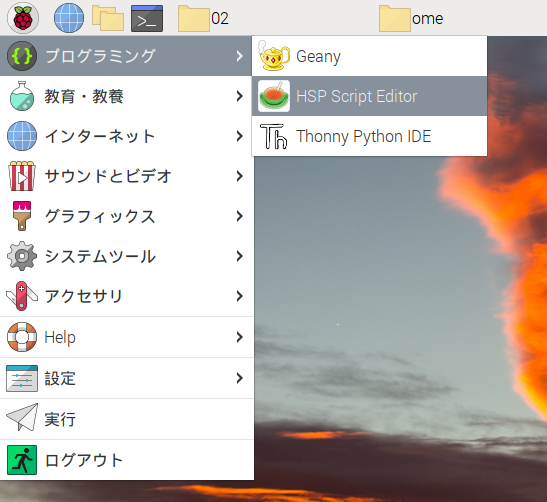
\includegraphics[keepaspectratio,width=7.31cm,height=6.562cm]{../../asset/image/s_hspmenu.png}
      \caption{プログラミング項目のメニュー}
    \end{center}
\end{figure}


いつも通りに、HSPスクリプトエディタを起動して作業を始めていきましょう。

\begin{figure}[H]
    \begin{center}
      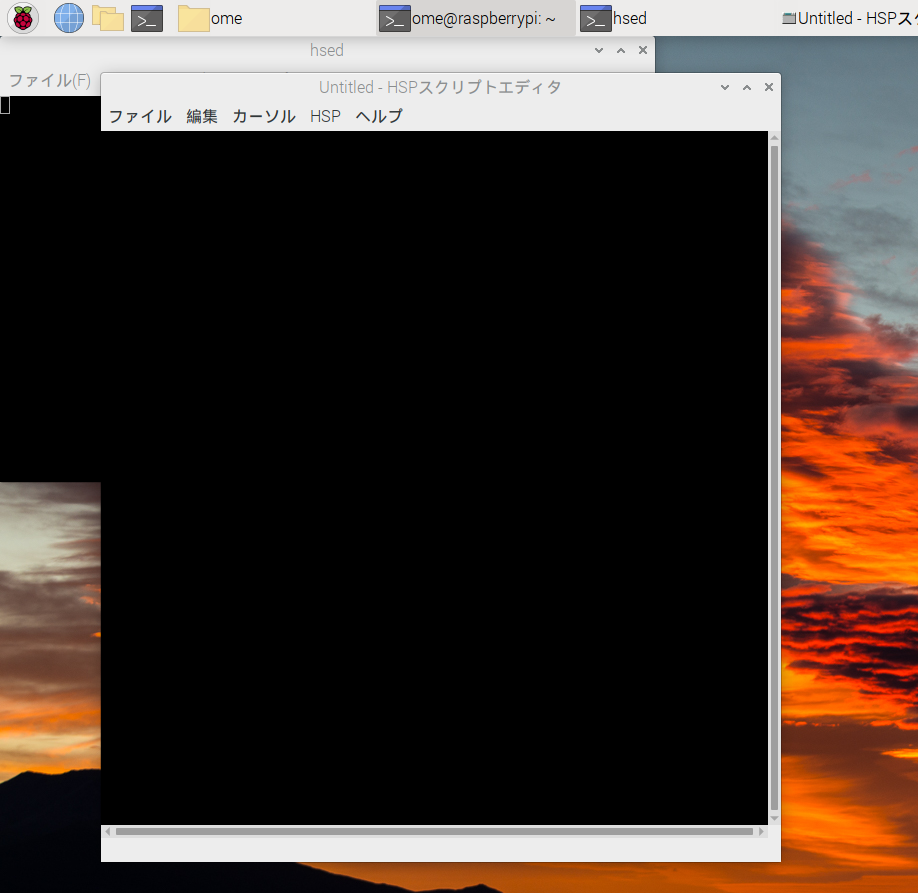
\includegraphics[keepaspectratio,width=7.31cm,height=6.562cm]{../../asset/image/s_hsed.png}
      \caption{HSPスクリプトエディタを起動したところ}
    \end{center}
\end{figure}
\clearpage



まずは、プログラムを動かして試してみましょう。

ファイル→「開く」メニューから /home/ユーザー名/04 フォルダの中にある「swhandan.hsp」を読み込んでください。
作業は、すべて「/home/ユーザー名/04」フォルダで行ないます。

見つからない場合は、まわりの友達か、近くの先生に聞いてみてください。


\begin{figure}[H]
    \begin{center}
      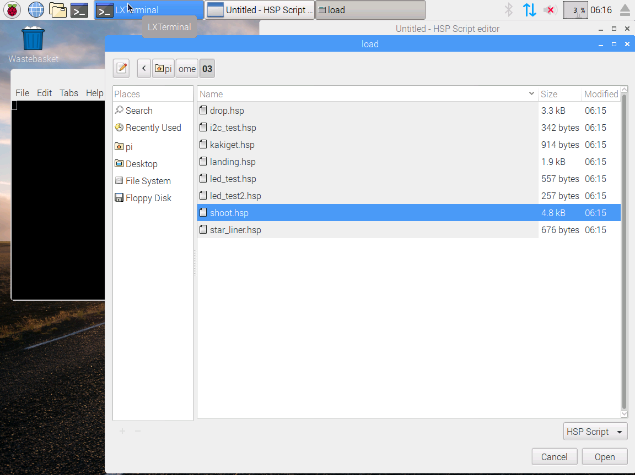
\includegraphics[keepaspectratio,width=7.338cm,height=5.493cm]{../../asset/image/s_loadfile.png}
      \caption{フォルダから読み込む画面}
    \end{center}
\end{figure}


「swhandan.hsp」は、センサーボード上のスイッチを押すとメッセージが\ruby{変}{か}わるかんたんなプログラムです。まずは、[F5]キーを押して\ruby{実行}{じっ|こう}してみましょう。
%330


\begin{figure}[H]
    \begin{center}
      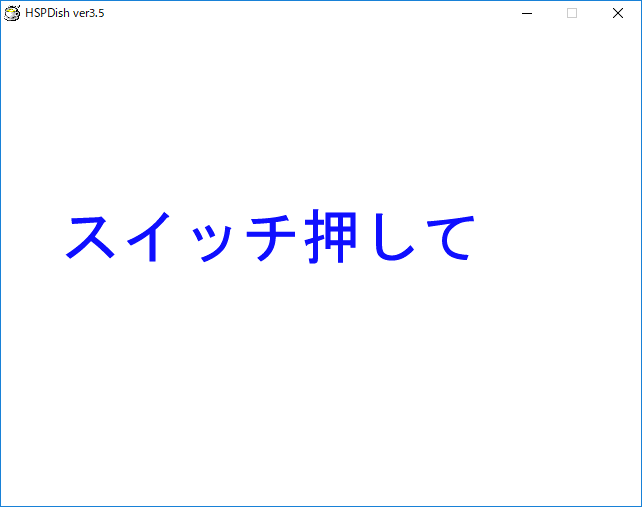
\includegraphics[keepaspectratio,width=7.673cm,height=6.05cm]{../../asset/image/s_swhandan.png}
      \caption{swhandan.hspの実行画面}
    \end{center}
\end{figure}


%347
%350

第2回で出てきた条件判断について思い出してみましょう。

プログラムは最初の行から、下に向かって\ruby{順番}{じゅん|ばん}に実行されます。\ruby{実際}{じっ|さい}には、\ruby{一瞬}{いっ|しゅん}ですぎてしまうのでわかりにくいですが、どのような順番でコンピューターが動くのか、想像しながら見てみることが大切です。わからない命令は以前の教科書を復習してみましょう。
\clearpage

「*hata」から「goto *hata」までの\ruby{間}{あいだ}が「スイッチ押して」という文字を\ruby{表示}{ひょう|じ}する部分です。




\begin{lstlisting}[firstnumber=3]
*hata
    redraw 0
    font "",60
    pos 60,180
    color 0,0,255
    mes "スイッチ押して"
    redraw 1
    await 16
    if gpioin(5)=0 : goto *hata2
    goto *hata
\end{lstlisting}

ここでセンサーボードのスイッチを押すと流れが変わります。

\begin{lstlisting}[firstnumber=14]
*hata2
    redraw 0
    font "",60
    pos 60,180
    color 255,0,0
    mes "押しましたね!"
    redraw 1
    await 16
    if gpioin(6)=0 : goto *hata
    goto *hata2
\end{lstlisting}


「*hata2」から「goto *hata2」までの間で「押しましたね」という文字を表示しています。

それぞれの\ruby{切}{き}り\ruby{替}{か}えにスイッチを使っていますが、そのために条件判断を使っています。

スイッチの\ruby{状態}{じょう|たい}などを知る\ruby{場合}{ば|あい}は、gpioinという\ruby{関数}{かん|すう}を使います。



\deschspsyntax{変数 = gpioin(GPIO番号)}

と書くことで、指定されたGPIO番号のスイッチがONかOFFかを調べることができます。

%444


\begin{figure}[H]
    \begin{center}
      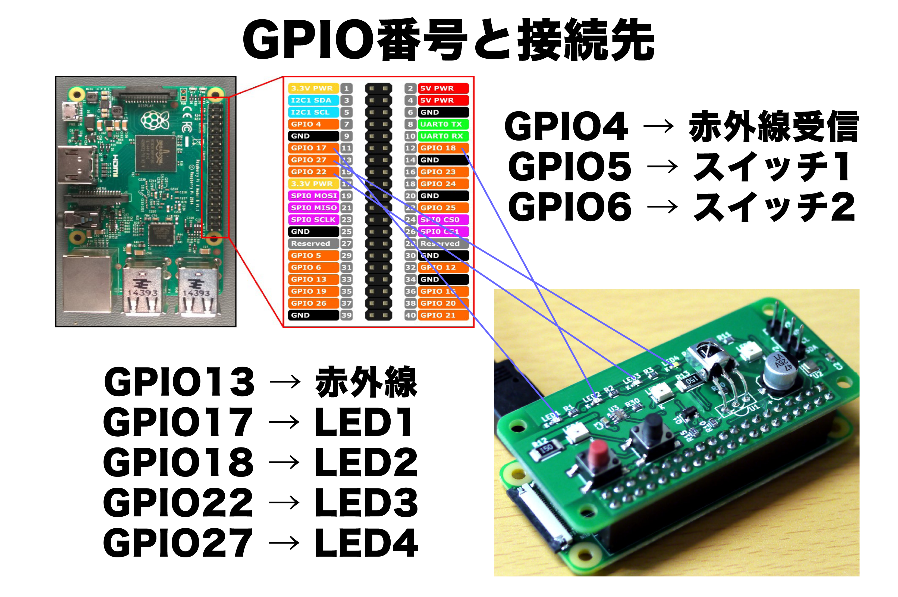
\includegraphics[keepaspectratio,width=12.409cm,height=7.62cm]{../../asset/image/s_gpio.png}
    \end{center}
\end{figure}



スイッチが接続されているGPIOの番号を指定することで\ruby{変数}{へん|すう}に値を入れることができます。

\begin{lstlisting}[numbers=none]
    a = gpioin(5)
\end{lstlisting}

と書くことで、スイッチ1がONならば0、OFFならば1が変数に代入されます。

変数に記憶されている0か1の数字をもとに、条件判断で違う動作をさせることができます。

条件判断のための if命令 を思い出してみましょう。

%478

\begin{itembox}[c]{HSPのルール}
    if命令により条件を判断することができます。ifの後にスペースに続けて条件式を指定します。その後で「:」に続けて条件が正しい時に実行される命令を書きます。
\end{itembox}

\begin{center}
    (条件式はいくつか書き方があります)
\end{center}
\begin{center}
    \begin{tabular}{cl} \hline
        条件式 & 意味 \\ \hline
        変数名 = 数値 & 変数の内容と数値が同じである \\
        変数名 ! 数値 & 変数の内容と数値が同じではない \\
        変数名 {\textless} 数値 & 変数の内容より数値の方が数が大きい \\
        変数名 {\textgreater} 数値 & 変数の内容より数値の方が数が小さい \\ \hline
    \end{tabular}
\end{center}

つまり、


\begin{lstlisting}[numbers=none]
    a = gpioin(5)
    if a=0 : goto *hata
\end{lstlisting}


のように書くことで、変数aが0の時だけ「*hata」の場所から実行させることができます。

(センサーボードのスイッチは押された時に0の値になります。1ではないので注意しましょう。)
\end{document}
